\label{chap6}
To be able to evaluate the proposed solution in a real-life scenario, a prototype based on the concept presented was built. This chapter introduces the implementation from a high level
view, followed by the evaluation of the result. Afterwards, the results are discussed and improvements are suggested.
\section{Implementation}
\subsection{Bus interface}
The necessary software, running on each platform, is written in the programming language "C". To interface with \gls{knx}, an \gls{api} named \gls{eibd} is used, providing functions to
send \gls{knx} frames to and receive frames from the bus. \gls{eibd} offers synchronous as well as asynchronous calls for sending and receiving frames. While the first kind of
call will block until the operation finished, the second kind of call will return immediately, the status of such calls can be checked by another special \gls{eibd} call.
Because it is not possible to use callbacks with asynchronous calls, the implementation uses the synchronous functions.

\subsection{Concurrency}
Every platform possess 3 distinct interfaces to the bus (2 interfaces form the redundant "secure" part of the network, one is connected
to a standard \gls{knx} network), so care must be taken that no frames are missed or delayed due to a blocking call to \gls{eibd}. This can be achieved by splitting the main program into different 
processes or alternatively, threads, where for each critical task, a distinct part is responsible. While threads share the same address space, facilitating communication with
each other, processes rely on special system calls 
to share information. Additionally, thread-creation and switching between threads consumes less computing resources. Therefore, it was decided to choose the multi-threaded
approach. Consequently, at least 3 different threads - one for each communication interface - are needed. Nevertheless, because every thread must be able to write to \textit{or} receive
frames from the bus at unpredictable moments, 7 different threads are used: the main thread only handles argument processing and creates the other threads. For the remaining threads,
two pairs are responsible for the interfaces to the secured network, while the remaining thread pair handles writing to and reading from the bus. This setup is shown in
Figure \ref{fig:threads}.
\begin{figure}[h]
\centering
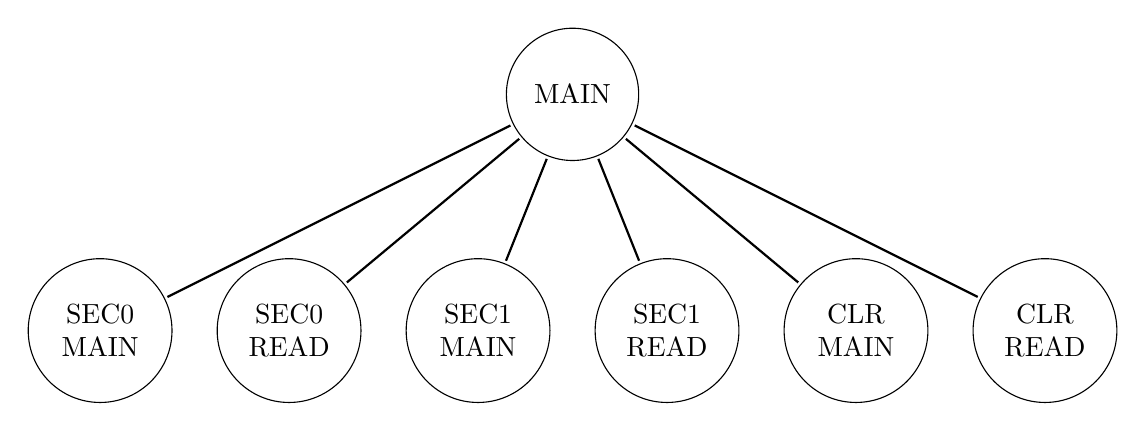
\begin{tikzpicture}[scale=0.2]
\tikzstyle{every node}+=[inner sep=2pt]
\tikzstyle{arrow}=[draw, -latex] 
\tikzset{
    pil/.style={
           ->,
           thick,
           shorten <=1pt,
           shorten >=1pt,}
}
\usetikzlibrary{automata,positioning}
\usetikzlibrary{positioning}
\node[state,text width=1.5cm,align=center]					at (-10,5)		(m)			{MAIN}; 
\node[state,text width=1.5cm,align=center]					at (-40,-10)	(sec0m)	{SEC0 MAIN}; 
\node[state,text width=1.5cm,align=center]					at (-28,-10)	(sec0r)		{SEC0 READ}; 
\node[state,text width=1.5cm,align=center]					at (-16,-10)	(sec1m)	{SEC1 MAIN}; 
\node[state,text width=1.5cm,align=center]					at (-4,-10)		(sec1r)		{SEC1 READ}; 
\node[state,text width=1.5cm,align=center]					at (8,-10)	(clrm)		{CLR MAIN}; 
\node[state,text width=1.5cm,align=center]					at (20,-10)	(clrr)			{CLR READ};
\path[pil,-] (m)  edge[auto]   node[] {} (sec0m); 
\path[pil,-] (m)  edge[auto]   node[] {} (sec0r); 
\path[pil,-] (m)  edge[auto]   node[] {} (sec1m); 
\path[pil,-] (m)  edge[auto]   node[] {} (sec1r); 
\path[pil,-] (m)  edge[auto]   node[] {} (clrm); 
\path[pil,-] (m)  edge[auto]   node[] {} (clrr); 

%\path[pil,->] (sec0r)  edge[auto, out=240, in=300]   node[] {} (sec0m); 
%\path[pil,->] (sec1r)  edge[auto, out=240, in=300]   node[] {} (sec1m); 
%\path[pil,->] (clrr)  edge[auto, out=210, in=290]   node[] {} (sec1m); 
%\path[pil,->] (clrr)  edge[auto, out=230, in= 180]   node[] {} (sec0m); 
\end{tikzpicture}
\label{fig:threads}
\caption{Threads used in the implementation}
\end{figure}
This design allows to assign one timing-critical task to every thread: every \textit{READ} thread immediately opens its corresponding bus interface in \textit{monitor} mode, allowing it
to read all the bus traffic on the corresponding line. After that, it enters a loop, performing a blocking read call to \gls{eibd} on every iteration.
This will set the whole thread to \textit{blocked}, and the operating
system will set another thread or process as runnable. Whenever data is available to the blocked thread, the operating system will buffer the received data and eventually set the
thread runnable again. Thus, no frames will be missed.
\\
\\
The main-threads of the secure lines (i.e. \textit{SEC0 MAIN} and \textit{SEC1 MAIN}) will start the synchronization sequence, as described in Section \ref{syncService}, and send out
the synchronization messages. After  that, the main threads will enter the \textit{READY} state and listen for discovery messages.
\\
\\
Whenever the \textit{CLR READ} thread receives new data, the frame will be forwarded to booth \textit{SEC MAIN} threads together with the counter for the unique source address, contained
in the frame. Booth \textit{SEC MAIN} threads will send discovery requests, independently from each other, each containing newly chosen \gls{ecdh} parameters. Responsible gateways (i.e.
gateways which are connected to the wanted destination address through their cleartext lines) will compute a new \gls{ecdh} parameter, derive distinct shared secrets for booth lines,
save them and send the parameters contained in the discovery responses back to the requesting device. The requester than derives the same shared secrets, and sends the encrypted frame,
contained in extended \gls{knx} frames, to the destination gateways, which will check and decrypt them and forward booth decrypted frames and the corresponding global counter values
to the \textit{CLR MAIN} thread. Here, the duplicate will be discarded and one frame will be sent to its final destination.
\\
\\
A thread can be created in C with the function \textit{pthread\_create()}. The function expects 4 parameters:
\begin{itemize}
 \item a variable of type \textit{pthread\_t}
 \item attributes for the new thread, or NULL for default values
 \item a function pointer, serving as entry-point for the new thread
 \item parameters for the function pointer, or NULL
\end{itemize}
\begin{lstlisting}[style=BashInputStyle,caption={Thread-creation},label=lst:pthread_create]
if((pthread_create(&sec1MasterThread, NULL, (void *)secMasterStart, &threadEnvSec[0])) != 0)
        {
                printf("sec1Thread thread init failed, exit\n");
                return -1;
        }
\end{lstlisting}

\subsection{Thread-to-thread communication}
To pass data from one thread to another, different ways are possible. While the easiest way would be to use global data structures, the implementation uses 
\gls{posix}-pipes instead, mainly because with pipes, timeouts can be implemented easily. Such timeouts are used when waiting for synchronization replies, as well as for 
cleanup tasks.
\\
A new pipe is created as shown in Listing \ref{lst:pipe}.
\begin{lstlisting}[style=BashInputStyle,caption={Creating a pipe},label=lst:pipe]
int pipefd[2];
...
if(pipe(pipefd) == -1)
{
  printf("pipe() failed, exit\n");
  exit(-1);
}
\end{lstlisting}
Every pipe possess two file descriptors, providing a uni-directional data channel: data can be written to the pipe by performing a write() - operation to the \textit{write}-end of the
pipe, while the data can be read from the pipe by calling read() with the \textit{read}-end of the pipe. Basically, the read() operation will block until new data can be read - in 
combination with the select() system call, a maximum time for the blocking operation can be set, as shown in Listing \ref{lst:timeout}
\begin{lstlisting}[style=BashInputStyle,caption={Creating a pipe},label=lst:timeout]
fd_set set;
struct timeval timeout;
int selectRC;
...
FD_ZERO(&set);
FD_SET(fileDescriptor, &set);
timeout.tv_sec = 2;	// set timeout to 2 seconds
timeout.tv_usec = 0;
selectRC = select(FD_SETSIZE, set, NULL, NULL, timeout);
if(selectRC == 0)
{
   // timeout occured
}
else if(selectRC < 0)
{
  // error occured
}
else
{
  // data received - read it:
  read(fileDescriptor, buffer, len);
}
\end{lstlisting}
In this example, FD\_ZERO at first clears the set containing the file handles to be watched, FD\_SET() then adds the file handle we are interested in (allowing to watch multiple file
descriptors). The timeout is then set to two seconds 
(microseconds granularity is supported, nevertheless the timing precision is limited by the system clock granularity and kernel scheduling delays), and select() is called. If no data is
received within 2 seconds, the if-branch is executed. If data is received in time, the else-branch is executed instead, and the waiting data can be obtained by performing a standard
read() call.

\subsection{Race conditions}
Software race conditions occur whenever an application, using shared resources, depends on the timing of its processes or threads.
Because the exact time when a particular process or thread is scheduled by the processor is unknown in advance, such conditions must be avoided.
An example of a program containing a race condition would be as following:
\begin{lstlisting}[style=BashInputStyle,caption={Race condition},label=lst:raceCond]
for ( int i = 0; i < 1000000; i++ )
{
   x = x + 1; 
}
// x = 1000000 ?
\end{lstlisting}
For a single-threaded program, this would produce the value $x=1000000$ after the loop, while for a 2-threaded program, the resulting value will depend on the exact scheduling of the
threads and very likely differ from the expected value $x=2000000$. The reason is that the statement incrementing x is no atomic operation. Instead, the operation will consist of
several statements on machine language level, forming a \textit{critical region}:
\begin{enumerate}
 \item load value from address into register
 \item add 0x01 to the register
 \item write value from register to address
\end{enumerate}
If thread 1 gets interrupted after the second step and thread 2 afterwards finishes, thread 1 will overwrite the value just written by thread 2 and thus produce a false result.
\\
\\
Such a critical region must be protected such that only one thread can enter it, a requirement also called \textit{mutex}, short for \textit{mut}ual \textit{ex}clusion.
The implementation uses the \gls{posix} \textit{pthread mutex} to lock critical regions, as shown in listing \ref{lst:mutex}:  
\begin{lstlisting}[style=BashInputStyle,caption={Locking a critical region},label=lst:mutex]
if(pthread_mutex_init(&globalMutex, NULL) != 0)
{
  printf("mutex init failed, exit");
  return -1;
}
pthread_mutex_lock(&globalMutex);
/*
    CRITICAL REGION
*/
pthread_mutex_unlock(&globalMutex);
\end{lstlisting}
\textit{globalMutex} is a global variable of type \textit{pthread\_mutex\_t}. After calling pthread\_mutex\_lock(), there are two possibilities: if the mutex is unlocked, the call will
lock it and continue the program flow. If it is already locked, the call to pthread\_mutex\_lock() will block. If the mutex is unlocked by the possessing thread, the blocked thread will
be set active, lock for his part and continue execution.\footnote{Of course, pthread\_mutex\_lock() must be executed in an atomic way, otherwise introducing a race condition on another
level}

\subsubsection{KNX addressing scheme}

Care must be taken that no duplicate \gls{knx} addresses are used within the network. Therefore, the following addressing convention is proposed:
While it would be possible to use the same addresses on both lines per gateway, a different scheme is used.
For the secured network, the address ranges starting at address 1.1.1 to address 1.1.15 and 1.2.1 to 1.2.15 are reserved for secure line number
1 and 2 respectively, which allows a maximum of 15 gateways. Different addresses are used mainly because it facilitates debugging. 
On the unsecured lines, every gateway uses an address from the range 1.0.1 - 1.0.15. Addresses are assigned in a linearly ascending way, so gateway number 1
uses addresses 1.1.1 and 1.2.1 for secure lines 1 and 2, and 1.0.1 for its unsecured line.

\subsection{\gls{mac2} generation}

The \gls{ttl} field cannot be included in the \gls{mac2} calculation because this field gets changed by a router and would therefor invalidate an authentic message.

\subsection{EIBD \gls{api}}

Use VBusMonitor to receive packets, this way EIBD can L2 acknowledge individual-, group- and broadcast frames
\\
\\
For sending individual packages, use EIBOpenT\_Individual(con, myAddr, FALSE)
\\
\\
For sending group packages, use EIBOpen\_GroupSocket(con, TRUE) and EIBSendGroup(con, dest, size, buf)
\\
\\
For sending broadcast packages, use EIBOpenT\_Broadcast(con, TRUE) and EIBSendAPDU(con, size, buf)

\subsection{Restrictions }

EIBD can send extended frames, but can not receive frames with payload >= 56 byte. 

\subsection{FIXMEs}

\begin{enumerate}
 \item DH: apply hashingfunction on derived secret to get 2 different keys(MAC, encrypt)
 \item 
\end{enumerate}



\section{Evaluation}

\subsection{\gls{usb}}
Unstable \gls{usb} connection, enumeration errors, to fix reboot hub

\subsection{Synchronization phase}
Packages in the synchronization phase are not encrypted, allowing a passive adversary to learn the value of the global counter value $Ctr_{global}$. Nevertheless,
this counter is only used to avoid deterministic encryption (see \ref{deterministicEnc}) and is of no use for the attacker.
\\
\\
Opening a window for tolerating timing deviations allows an active attacker to inject a captured synchronization response package within that time window.
Nevertheless, because the header is protected by a \gls{mac2}, the only way to inject a synchronization package is to use exactly the same frame as captured,
i.e. the same source address, which will be discarded because the the requesting device already finished the synchronization stage.
\\
Additionally, the counter value is of no use for the attacker, as described above.

\subsection{Discovery phase}

\subsection{Data transmission phase}


\subsection{High Level Cryptography Library}

\subsubsection{OpenSSL}

\begin{itemize}
 \item install libssl, libssl-dev
\end{itemize}

